\section[散射过程的一般描述]{散射过程的一般描述} \label{sec:08.01} % 
% \makebox[5em][s]{} % 短题目拉间距

{\heiti 1. 散射截面}

在弹性散射过程中,发生碰撞的两个粒子之间的相互作用可以用一个等效的势场$V$表示.在质心坐标系中,弹性散射过程相当于质量为$\mu$(二体问题中的折合质量)的粒子从远方入射,受势场$V(\boldsymbol{r})$作用而改变其运动方向(但能量不变),如图\ref{fig.8-1}所示.

\begin{figure}[!h]
	\centering
	\small
	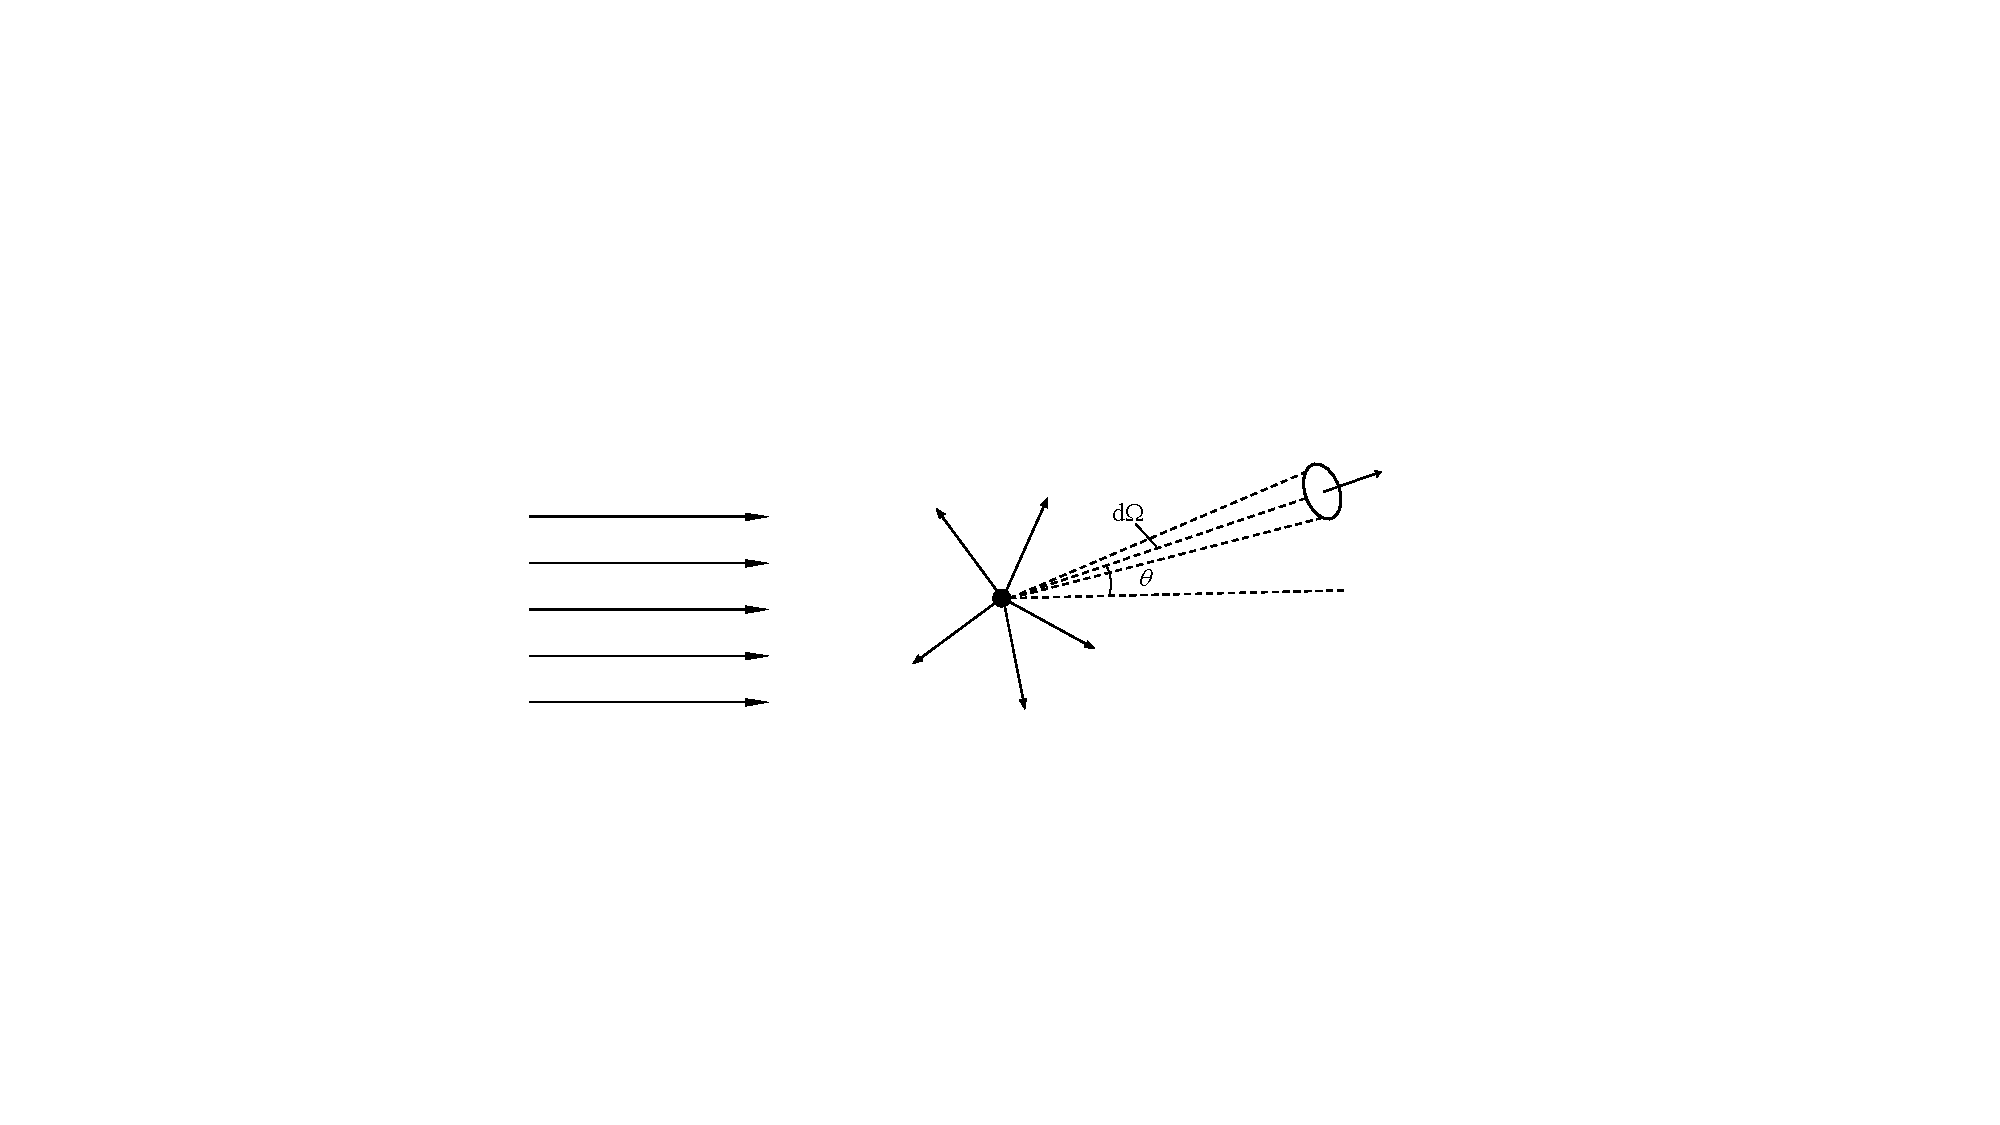
\includegraphics[width=6cm,clip]{QM file/figure/8-1}
	\caption{}\label{fig.8-1}
\end{figure}
粒子运动方向的偏转角称为散射角,即图中$\theta$.考虑一束速度为$v$的入射粒子,入射流量(入射方向单位横截面上,单位时间内通过的粒子数)为$N_{0}$,单位时间内散射的(改变了运动方向的)粒子数为$N$,其中散射到角范围$d\Omega$内的粒子数为$dN$.显然$N$与$dN$均和$N_{0}$成正比,令
\eqshort
\begin{empheq}{align}
	dN &= N_{0}\sigma(\theta,\varphi)d\Omega	\label{eq81.1}	\\
	N  &= \int dN=\sigma_{\text{总}}N_{0}		\label{eq81.2}
\end{empheq}
$\sigma(\theta.\varphi)$与$\sigma_{\text{总}}$的量纲均为面积,$\sigma_{\text{总}}$称为有效总散射截面,意义为,就散射的总效果而言,靶粒子(作用势$V$)相当于挡在入射粒子前进路上的一块横截面$\sigma_{\text{总}}$.$\sigma(\theta,\varphi)$称为有效微分散射截面,它和角元$d\Omega$所处的方向有关,其值取决于作用势$V$的性质.显然
\begin{empheq}{equation}\label{eq81.3}
	\sigma_{\text{总}}=\int\sigma(\theta,\varphi)d\Omega
\end{empheq}
在散射实验中,$N_{0}$和$dN/d\Omega$可以直接测量出来,再利用\eqref{eq81.1}式就得到$\sigma(\theta,\varphi)$的实验值,再由\eqref{eq81.3}式得到$\sigma$的实验值.散射理论的一项主要内容就是建立一套计算$\sigma(\theta,\varphi)$的理论方法,通过理论和实验的比较研究作用势$V$的性质.

{\heiti 2. 散射振幅}

作为散射过程的量子力学描述,入射粒子束可以近似地用平面波描述.以入射方向为$z$轴方向,入射粒子的动量表示成
\begin{empheq}{equation}\label{eq81.4}
	p=\mu v=\hbar k
\end{empheq}
则入射波为
\begin{empheq}{equation}\label{eq81.5}
	\varPsi_{i}=e^{ikz}
\end{empheq}\eqnormal
入射粒子数流量规定成
\begin{empheq}{align}\label{eq81.6}
	N_{0} &=j_{i}=-\frac{i\hbar}{2\mu}\bigg(\varPsi_{i}^{*}\frac{\partial}{\partial r}\varPsi_{i}-\varPsi_{i}\frac{\partial}{\partial r}\varPsi_{i}^{*}\bigg)	\nonumber\\
	&=\frac{\hbar k}{\mu}=v
\end{empheq}
($\varPsi_{i}^{*}\varPsi_{i}=1$,即规定单位体积内入射粒子数为1)
\noindent 散射过程的总波函数$\varPsi$可以表示成入射波$\varPsi_{i}$与散射波$\varPsi_{s}$之和,
\begin{empheq}{equation}\label{eq81.7}
	\varPsi=\varPsi_{i}+\varPsi_{s}=e^{ikz}+\varPsi_{s}
\end{empheq}
对于弹性散射,能量守恒,$\varPsi$满足定态薛定谔方程
\begin{empheq}{equation}\label{eq81.8}
	-\frac{\hbar^{2}}{2\mu}\nabla^{2}\varPsi+V(\boldsymbol{r})\varPsi=E\varPsi
\end{empheq}
其中$E=\frac{p^{2}}{2\mu}=\frac{\hbar^{2}k^{2}}{2\mu}$.通常,散射作用势$V$仅在小范围内起作用,$r\rightarrow\infty$处$V$迅速趋于0,这时\eqref{eq81.8}式变成自由粒子方程:
\begin{empheq}{equation}\label{eq81.9}
	\nabla^{2}\varPsi+k^{2}\varPsi\approx0\quad (r\rightarrow\infty)
\end{empheq}
入射波$\varPsi_{i}$是\eqref{eq81.9}式的一个严格解.$r\rightarrow\infty$处散射波$\varPsi_{s}$应该是\eqref{eq81.9}式的近似解,并取由散射中心$(r=0)$向外传播的球面波形式,即
\begin{empheq}{equation}\label{eq81.10}
	\varPsi_{s}\sim f(\theta,\varphi)\frac{e^{ikr}}{r}\quad (r\rightarrow\infty)
\end{empheq}
其中$f(\theta,\varphi)$称为散射振幅,它与方向$(\theta,\varphi)$有关.容易验证,当$r\rightarrow\infty$,如果略去$r^{-2}$以下小量,则不论$f(\theta,\varphi)$取什么函数形式,\eqref{eq81.10}式都能满足\eqref{eq81.9}式.这表明,在远离散射中心处$(r\rightarrow\infty)$,散射粒子又回到自由运动状态,\eqref{eq81.10}式正是自由粒子外向球面波波函数的一般近似表达式.(略去$r^{-2}$以下小量)一般需要解\eqref{eq81.8}式才能求得散射振幅$f(\theta,\varphi)$.

实验测量是在远离散射中心处进行的,相当于$r\rightarrow\infty$.如果略去$r^{-3}$以下小量,散射粒子数流量为
\begin{empheq}{align*}
	j_{s} &=-\frac{i\hbar}{2\mu}\bigg(\varPsi_{s}^{*}\frac{\partial}{\partial r}\varPsi_{s}-\varPsi_{s}\frac{\partial}{\partial r}\varPsi_{s}^{*}\bigg)	\\
	&=v|f(\theta,\varphi)|^{2}\bigg/ r^{2}
\end{empheq}
在角元$d\Omega$的横截面$r^{2}d\Omega$上单位时间内通过的散射粒子数为
\begin{empheq}{equation}\label{eq81.11}
	dN=j_{s}r^{2}d\Omega=v|f(\theta,\varphi)|^{2}d\Omega
\end{empheq}
与\eqref{eq81.1}式、\eqref{eq81.6}式比较,即得
\begin{empheq}{equation}\label{eq81.12}
	\sigma(\theta,\varphi)=|f(\theta,\varphi)|^{2}
\end{empheq}
散射理论的一项基本内容就是设法求出散射振幅$f(\theta,\varphi)$,从而算出微分散射截面$\sigma(\theta,\varphi)$.

{\heiti 3. 散射过程的经典力学描述}

在经典力学中,每个粒子均有一条运动轨道.以中心力场$V(r)$造成的散射为例,粒子的运动轨迹是一条平面曲线($\varphi$角不变),入射方向与出射方向的夹角就是散射角$\sigma$,如图\ref{fig.8-2}所示.散射角$\sigma$由碰撞参数(瞄准距离)$\rho$决定.经由横截面元$|\rho d\varphi d\rho|$的入射粒子,散射后进入$\theta$方向附近$d\Omega$角范围内,亦即
\begin{empheq}{equation}\label{eq81.13}
	dN=N_{0}|\rho d\rho d\varphi|=N_{0}\sigma(\theta)|d\Omega|
\end{empheq}

\begin{figure}[!h]
	\centering
	\small
	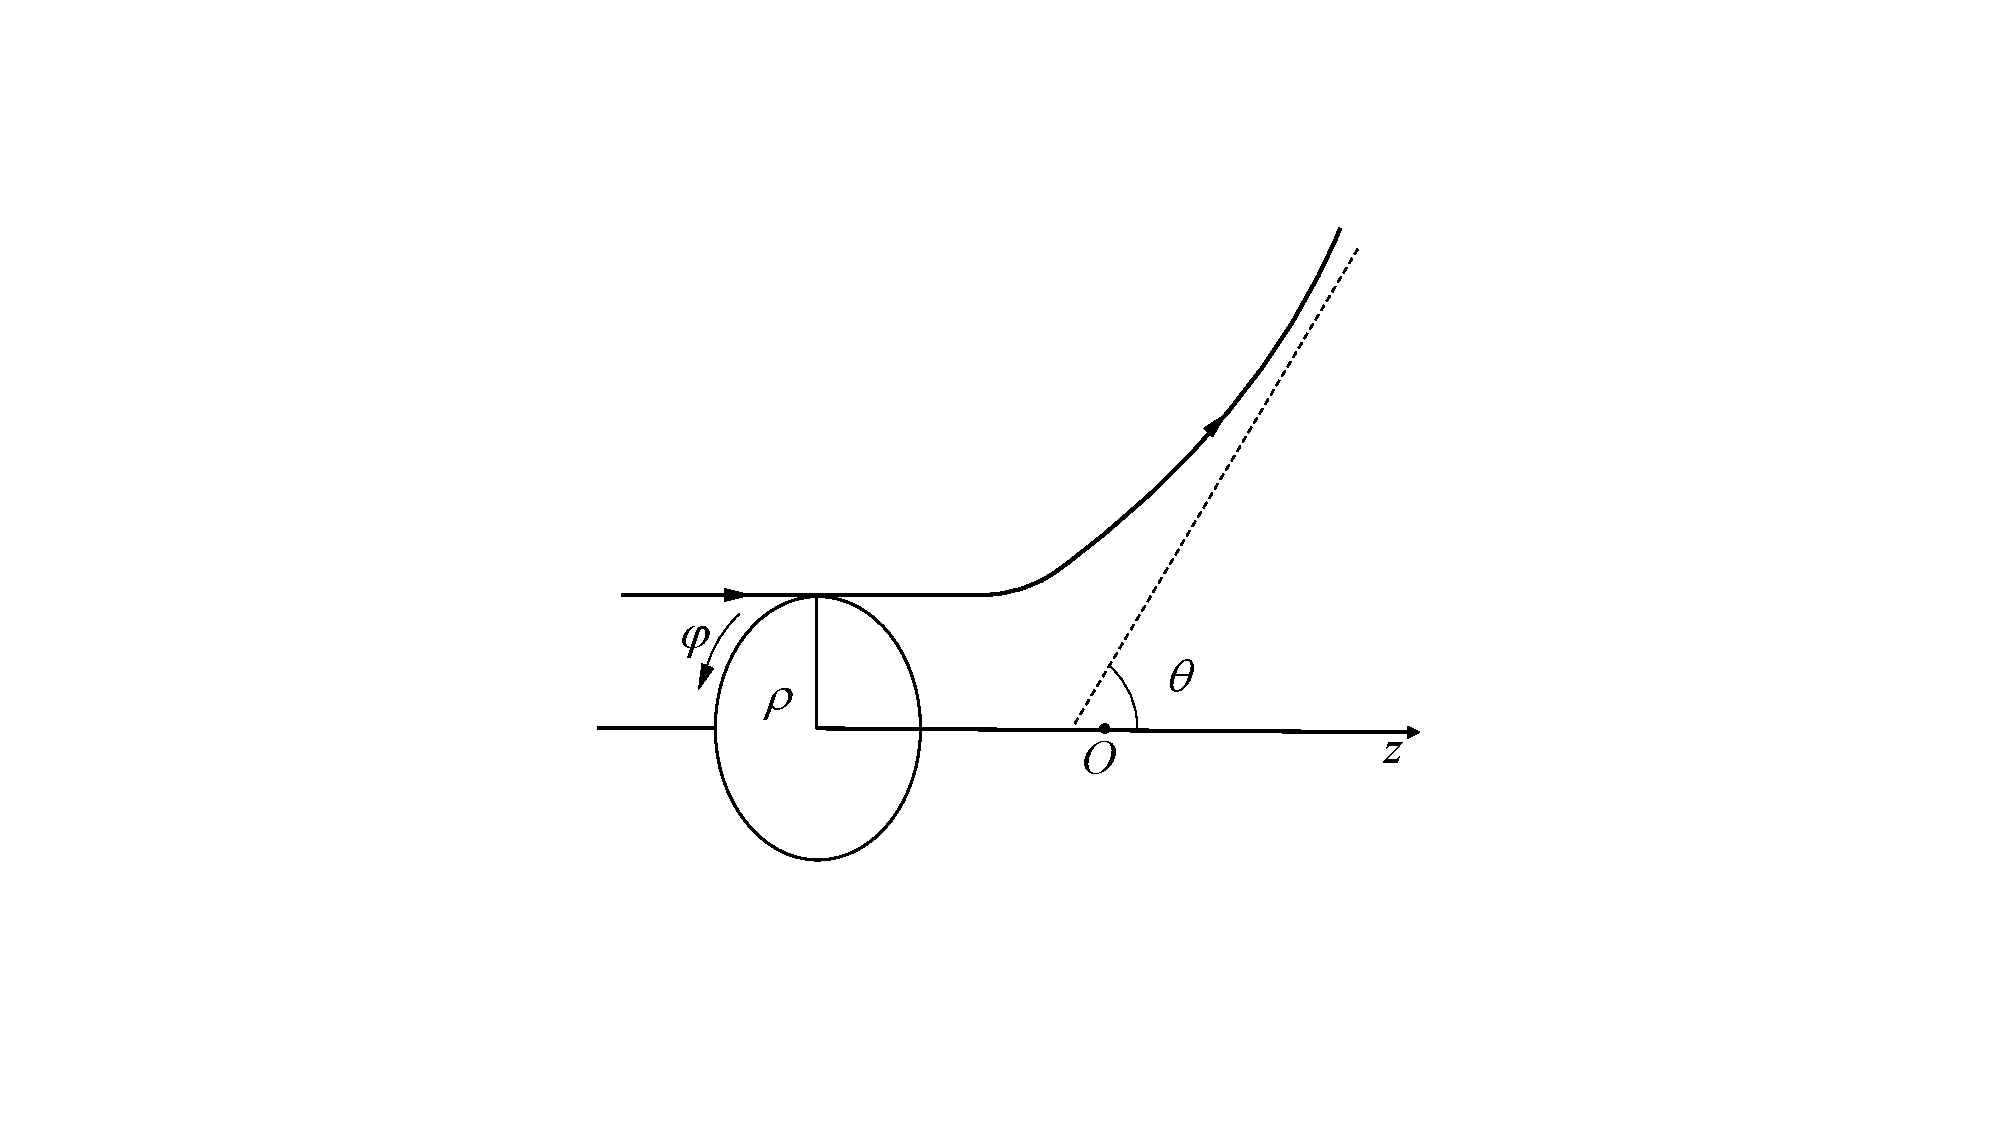
\includegraphics[width=4cm,clip]{QM file/figure/8-2}
	\caption{}\label{fig.8-2}
\end{figure}
其中$d\Omega=\sin\theta d\theta d\varphi$.由上式可得微分散射截面$\sigma(\theta)$的经典力学公式
\begin{empheq}{equation}\label{eq81.14}
	\sigma(\theta)=\left|\frac{\rho d\rho}{\sin\theta d\theta}\right|		%\bigg|\frac{\rho d\rho}{\sin\theta d\theta}\bigg|
\end{empheq}
经典散射理论的核心问题就是求碰撞参数$\rho$与散射角$\theta$的函数关系,从而得到$\sigma(\theta)$的公式.
\pskip

\example 速度为$v$的粒子束被半径为$a$的刚体球散射,求经典弹性散射截面.

\solution 总散射截面显然等于刚球的几何截面$\pi a^{2}$.下面求微分散射截面$\sigma(\theta)$.粒子与刚球碰撞发生弹性散射,入射角等于反射角,由图\ref{fig.8-3}容易看出下列关系:

\begin{figure}[!h]
	\centering
	\small
	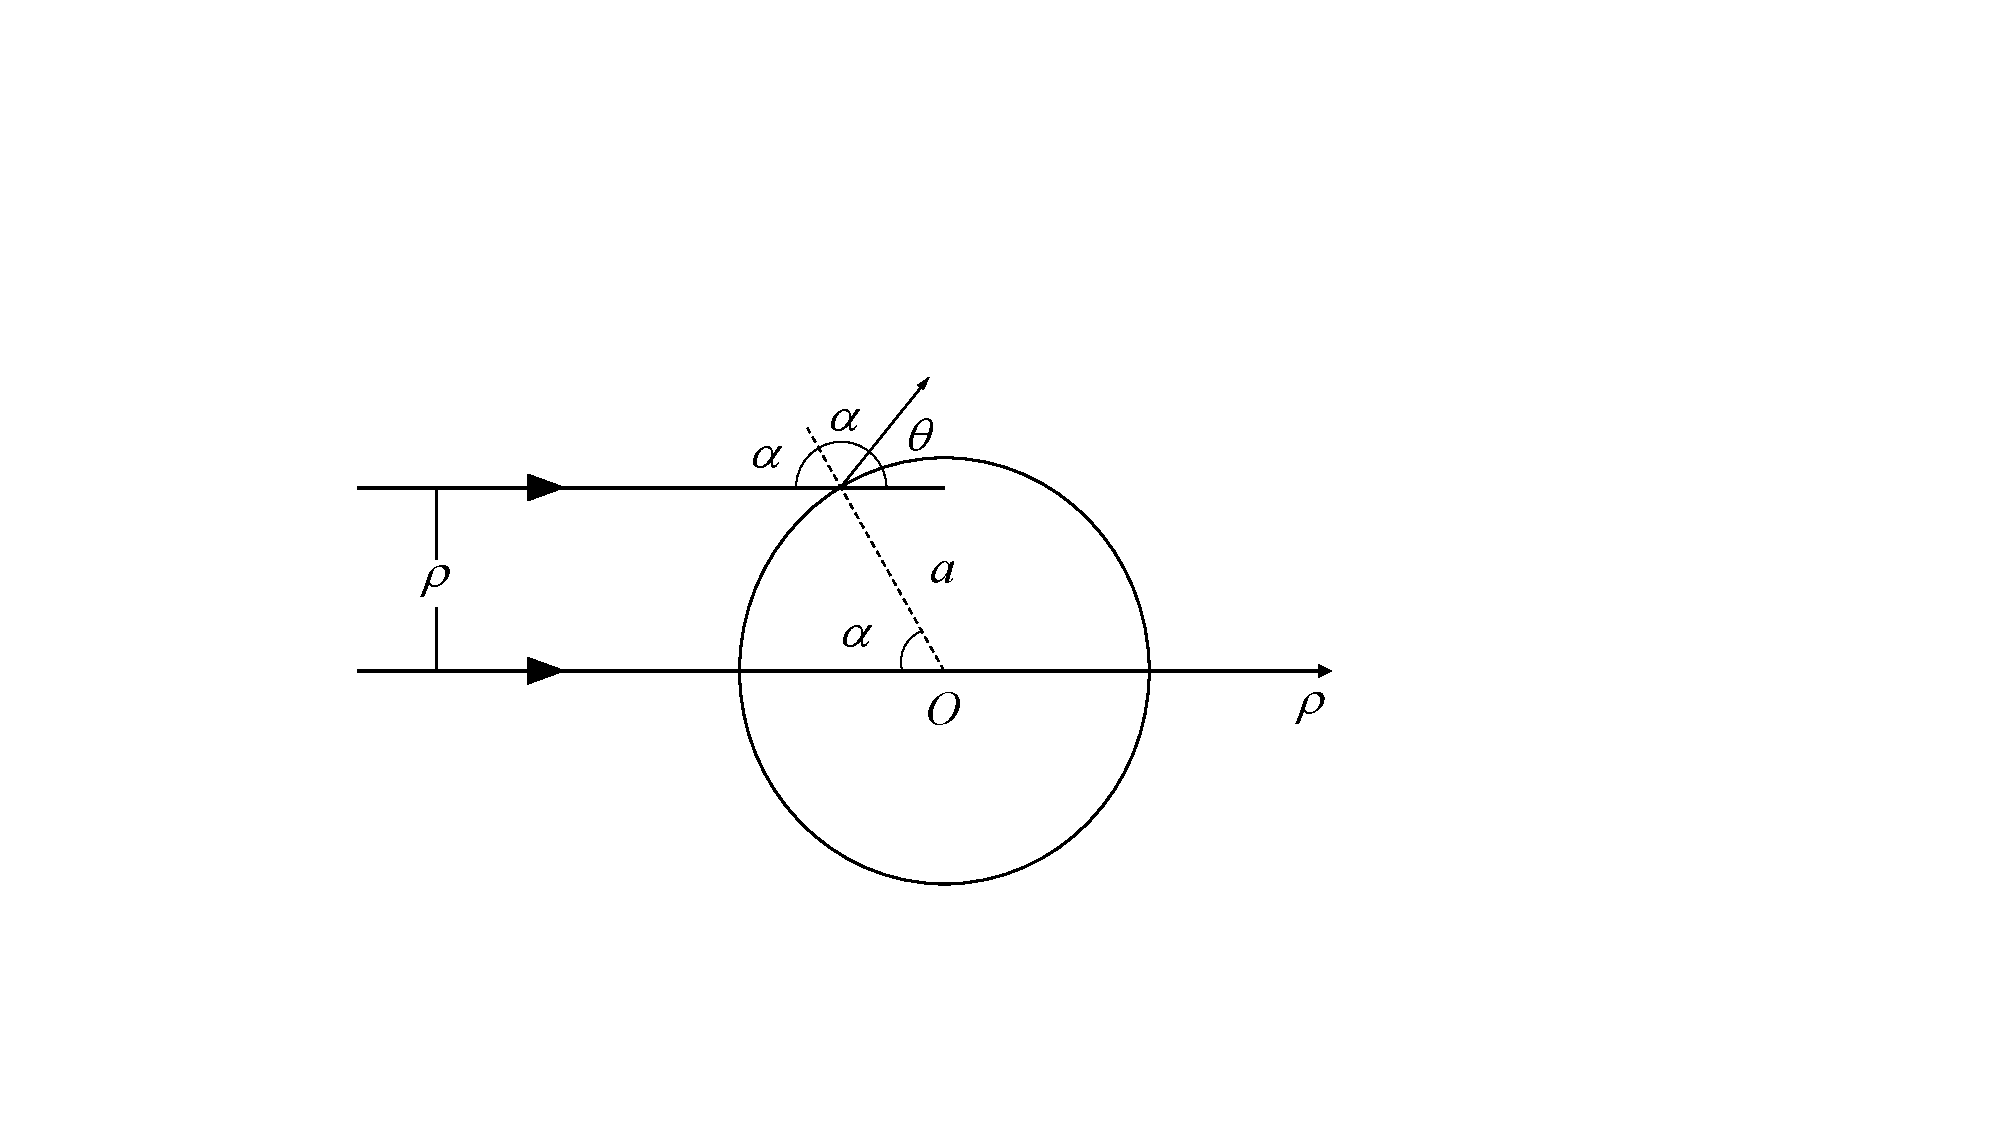
\includegraphics[width=5cm,clip]{QM file/figure/8-3}
	\caption{}\label{fig.8-3}
\end{figure}

\eqshort
\begin{empheq}{align*}
	&\theta+2\alpha=\pi	\\
	\rho= &a\sin\alpha=a \cos\frac{\theta}{2}
\end{empheq}\eqnormal
因此
\begin{empheq}{align*}
	\rho d\rho &=-\frac{a^{2}}{2}\cos\frac{\theta}{2}\sin\frac{\theta}{2}d\theta	\\
	&=-\frac{a^{2}}{4}\sin\theta d\theta
\end{empheq}
代入\eqref{eq81.14}式,即得
\eqshort
\begin{empheq}{equation}\label{eq81.15}
	\sigma(\theta)=a^{2}/4
\end{empheq}\eqnormal
$\sigma(\theta)$与$\theta$无关,这表示散射是各方向均匀的.显然
\begin{empheq}{align}\label{eq81.16}
	\sigma_{\text{总}} &=\int\sigma(\theta)d\Omega	\nonumber\\
		&= 4\pi\sigma(\theta)=\pi a^{2}
\end{empheq}

